\documentclass[12pt]{article} 

\usepackage{tikz}
\usetikzlibrary{patterns}
\pgfdeclarepatternformonly{south west lines}{\pgfqpoint{-0pt}{-0pt}}{\pgfqpoint{3pt}{3pt}}{\pgfqpoint{3pt}{3pt}}{
    \pgfsetlinewidth{0.4pt}
    \pgfpathmoveto{\pgfqpoint{0pt}{0pt}}
    \pgfpathlineto{\pgfqpoint{3pt}{3pt}}
    \pgfpathmoveto{\pgfqpoint{2.8pt}{-.2pt}}
    \pgfpathlineto{\pgfqpoint{3.2pt}{.2pt}}
    \pgfpathmoveto{\pgfqpoint{-.2pt}{2.8pt}}
    \pgfpathlineto{\pgfqpoint{.2pt}{3.2pt}}
    \pgfusepath{stroke}}
\usepackage[compat=1.1.0]{tikz-feynman}


\begin{document}


\begin{figure}[ht]
    \centering
    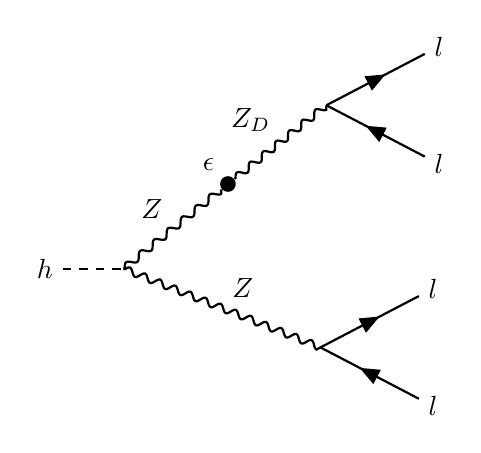
\begin{tikzpicture}

    \begin{feynman}[large]
        \vertex (h) {$h$}; % h at beginning 
        \vertex [right=1cm of h] (ZZ); % h -> ZZ vertex
        \node [circle, fill=black, inner sep=2pt, above right = 1cm and 1.25cm of ZZ] (Z1); % black dot node at epsilon (control size with ) 
        \node [above left = 7pt and 7pt of Z1] (e) {$\epsilon$}; % node with epsilon text
        \vertex [below right = 1cm and 2.5cm of ZZ] (Z2); % h -> ZZ bottom Z
        \vertex [above right = 0.5cm and 1.25cm of Z2] (Z2l1) {$l$}; % bottom Z -> ll (top l)
        \vertex [below right = 0.5cm and 1.25cm of Z2] (Z2l2) {$l$}; % bottom Z -> ll (bottom l)
        \vertex [above right = 1cm and 1.25cm of Z1] (ZD); % ZD
        \vertex [above right = 0.5cm and 1.25cm of ZD] (ZDl1) {$l$}; % ZD -> ll (top l)
        \vertex [below right = 0.5cm and 1.25cm of ZD] (ZDl2) {$l$}; % ZD -> ll (bottom l)
        
        \diagram* {
            (h) -- [scalar] (ZZ),
            (ZZ) -- [boson, edge label=$Z$] (Z1),
            (ZZ) -- [boson, edge label=$Z$] (Z2),
            (Z1) -- [boson, edge label=$Z_D$] (ZD),
            (ZDl2) -- [fermion] (ZD) -- [fermion] (ZDl1);
            (Z2l2) -- [fermion] (Z2) -- [fermion] (Z2l1);
        };
    \end{feynman}
    \end{tikzpicture}
\end{figure}

\newpage

\begin{figure}[ht]
    \centering
    \begin{tikzpicture}

    \begin{feynman}[large]
        \vertex (h) {$h$}; % h at beginning 
        \node [circle, fill=black, inner sep=2pt, right=1.5cm of h] (kappa); % black dot at kappa node
        \node [above left = 7pt and 7pt of kappa] {$\kappa$}; % node with kappa text
        \vertex [right=1.5cm of kappa] (s); % s -> ZDZD vertex
        \vertex [above right = 2cm and 1cm of s] (Z1); % top ZD
        \vertex [below right = 2cm and 1cm of s] (Z2); % bottom ZD
        \vertex [above right = 0.5cm and 1.25cm of Z2] (Z2l1) {$l$}; % top l of top Z
        \vertex [below right = 0.5cm and 1.25cm of Z2] (Z2l2) {$l$}; % bottom l of top Z
        \vertex [above right = 0.5cm and 1.25cm of Z1] (Z1l1) {$l$}; % top l of bottom Z
        \vertex [below right = 0.5cm and 1.25cm of Z1] (Z1l2) {$l$}; % bottom l of bottom Z
        
        \diagram* {
            (h) -- [scalar] (kappa),
            (kappa) -- [scalar, edge label=$s$, below] (s),
            (s) -- [boson, edge label=$Z_D$] (Z1),
            (s) -- [boson, edge label=$Z_D$] (Z2),
            (Z1l2) -- [fermion] (Z1) -- [fermion] (Z1l1);
            (Z2l2) -- [fermion] (Z2) -- [fermion] (Z2l1);
        };
    \end{feynman}
    \end{tikzpicture}
\end{figure}

\end{document}